\documentclass{beamer}
\usetheme[numbering=fraction, progressbar=frametitle]{metropolis}
\setbeamercovered{transparent}
\usepackage{pgfpages}
\setbeameroption{show notes on second screen=right}

\usepackage[utf8]{inputenc}
\usepackage[T1]{fontenc}
\usepackage{lmodern}
\usepackage{todonotes}
\usepackage{upgreek}

\graphicspath{{../Architektur/}}

\usepackage{templates/theme}

% configuration of slides
\titlelogo{FZI-Logo}								% logo on title slide and normal slides
%\titlelogo{none}
\setboolean{normallogo}{true}				% show title logo on normal slides?
\titlepicture{platine}						% picture on title slide
%\titlepicture{none}	
\setboolean{nav}{true}							% show navigation bar?
\setboolean{titlebar}{true}					% show green bar on title slide?
\setboolean{normalbar}{true}				% show green bar on normal slides?
\setboolean{normalcaptions}{true}		% show captions on normal slides?
\setboolean{innBW}{false}						% show innBW logo on normal slides?
\setboolean{minimalism}{true}			% minimalism mode? disables all the fancy things at once!

\title{Sensor Base Board\\ Für ein autonomes Boot}
\date{\today}
\author{Torben Mehner}
\subtitle{2M-Vortrag}
\institute{FZI, ESS}
\begin{document}
	
\begin{frame}
	\begin{titlepage}
		
	\end{titlepage}

	\vspace{30ex}

	{\color{fzi-gray} \scriptsize \hspace{-2ex}
	\begin{tabular}{l l}
		Betreuer: & Matthias Diehl \\
		& Friedrich Gauger \\
		Referent: & Prof. Dr. rer. nat W. Stork
	\end{tabular}}
\end{frame}

\begin{frame}{Inhaltsverzeichnis}
	\tableofcontents[sectionstyle=show,subsectionstyle=hide]
\end{frame}

%\section*{Einstieg}
%\begin{frame}
%	\begin{exampleblock}{}
%		{\LARGE ``The dinosaurs became extinct because they didn't have a space program.''}
%		\vskip5mm
%		\hspace*\fill{\small--- Larry Niven, Science-Fiction Autor}
%	\end{exampleblock}

%	\note{
%		Zum Einstieg ein Zitat von Larry Niven:
%	}
%\end{frame}

\section{Motivation}

\subsection{Stand der Technik}
\begin{frame}{\insertsection: \insertsubsection}
\begin{minipage}{0.45\linewidth}
	Stand der Technik
	\begin{itemize}
		\item Sonar-Geräte auf bemannten Booten
		\begin{itemize}
			\item Zeitverlust $\geq$ 5 min
			\item Slipstelle benötigt
		\end{itemize}
		\item Gefahr für Taucher
	\end{itemize}
	\note{
		Zeitverlust durch Slippen \\
		
		Abhängig von Position der Slipstellen \\
		
		Gilt, wenn Sonar zum Einsatz kommt \\
		Ansonsten suchen nur Taucher	
	}
\end{minipage} \quad
\begin{minipage}{0.45\linewidth}
	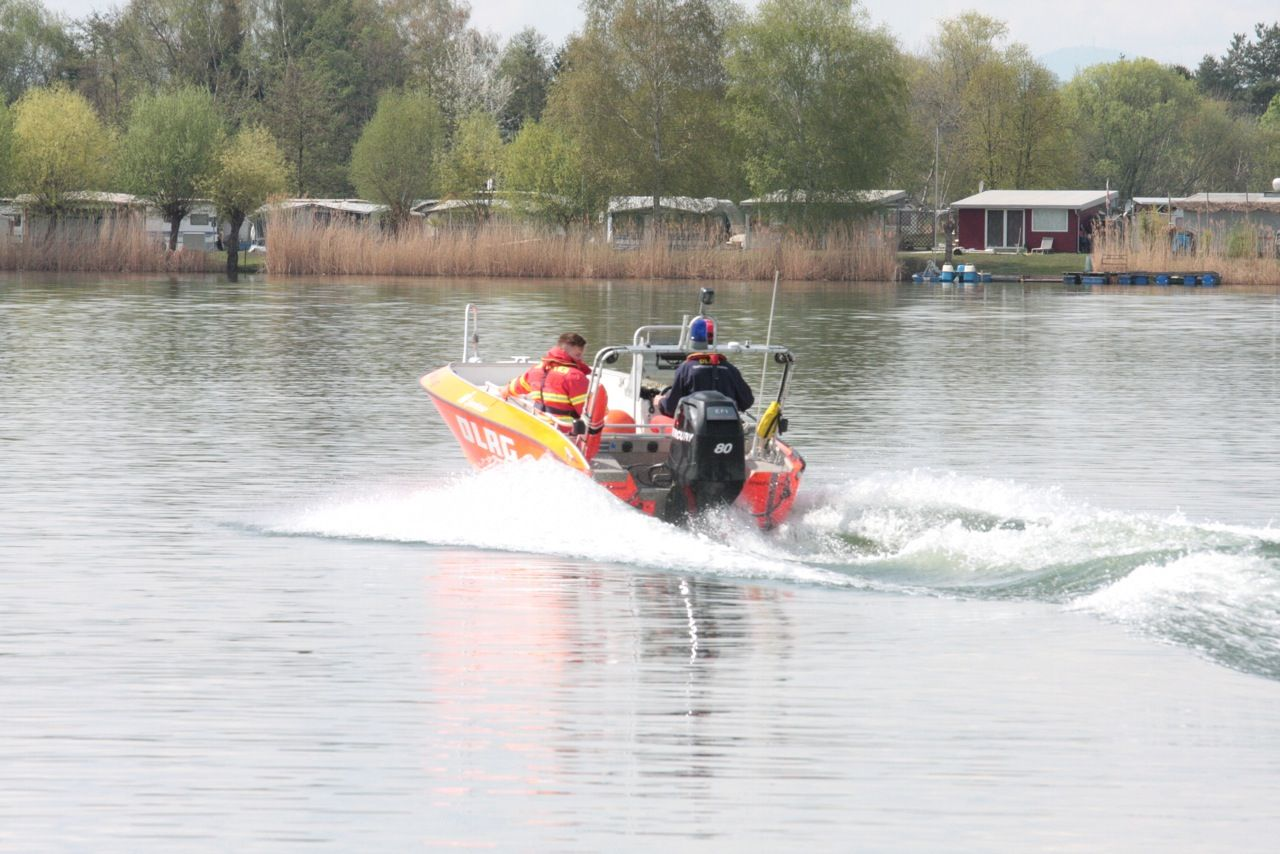
\includegraphics[width=\linewidth]{sonarboot}
\end{minipage}
\end{frame}

\subsection{Autonomes Boot}
\begin{frame}{\insertsection: \insertsubsection}
\begin{minipage}{0.45\linewidth}
	Autonomes Boot
	\begin{itemize}
		\item Unterstützt Rettungskräfte durch angebrachtes Sonar bei Personensuche
		\item Transportabel und schnell einsetzbar
		\item Fährt autonom Suchmuster
	\end{itemize}
\end{minipage} \quad
\begin{minipage}{0.45\linewidth}
	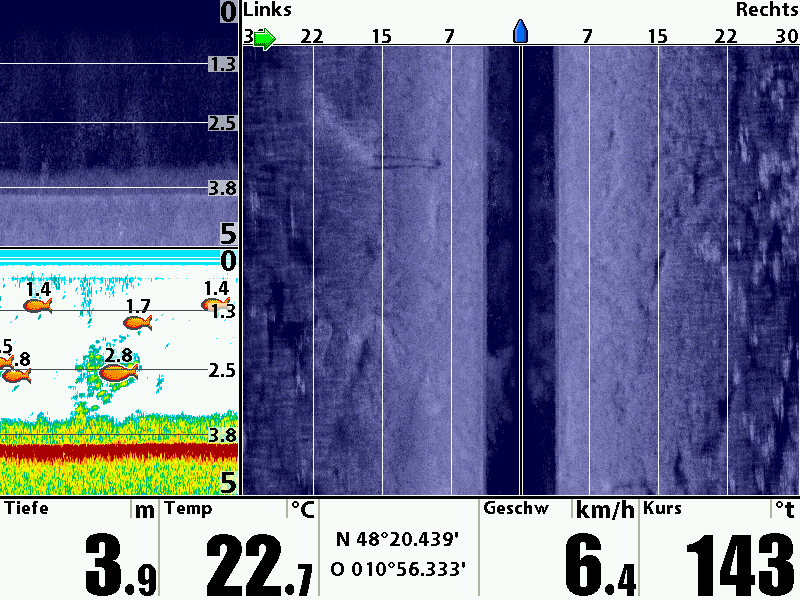
\includegraphics[width=\linewidth]{sonar}
\end{minipage}
\end{frame}

\subsection{SEC-Bike}
\begin{frame}{\insertsection: \insertsubsection}
\begin{minipage}{0.4\linewidth}
	Autonomes Lastfahrrad
	\begin{itemize}
		\item Wird per App bestellt
		\item Fährt autonom zu Ort
		\item Geschwindigkeit 6 km/h
	\end{itemize}
\end{minipage} \quad
\begin{minipage}{0.5\linewidth}
	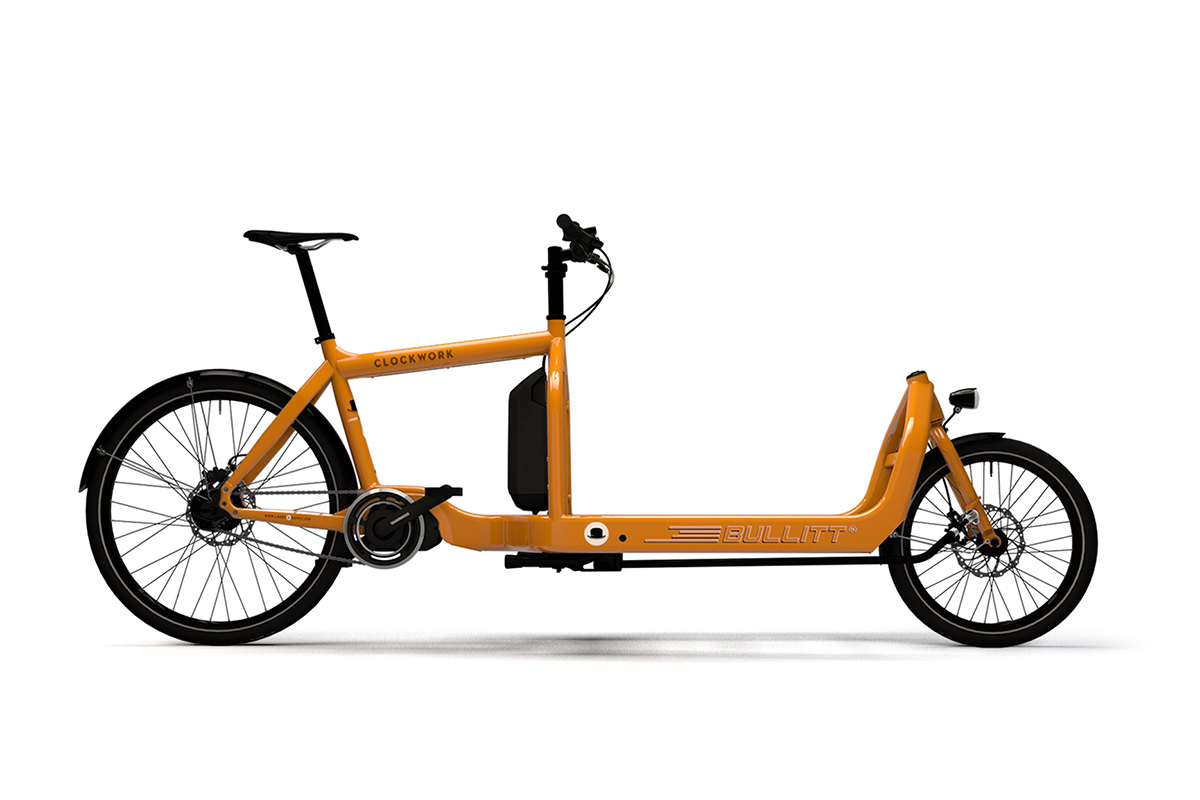
\includegraphics[width=\linewidth]{lastenrad}
	
	{\tiny Quelle: https://www.e-lastenrad.de/long-john/larry-vs-harry-steps-ebullitt}
\end{minipage}
\end{frame}

\subsection{Grundlagen}
\begin{frame}{\insertsection: \insertsubsection}
	Gemeinsame Fragen:
	\begin{itemize}
		\item Wo bin ich?
		\note{Selbstlokalisation}
		\item Wie komme ich zum Ziel?
		\note{Zielfindung}
		\item Wie komme ich dort sicher an?
		\note{Kollisionsvermeidung}
	\end{itemize}
\end{frame}

\section{Nötige Hardware}

\subsection{Überblick}
\begin{frame}{\insertsection: \insertsubsection}
	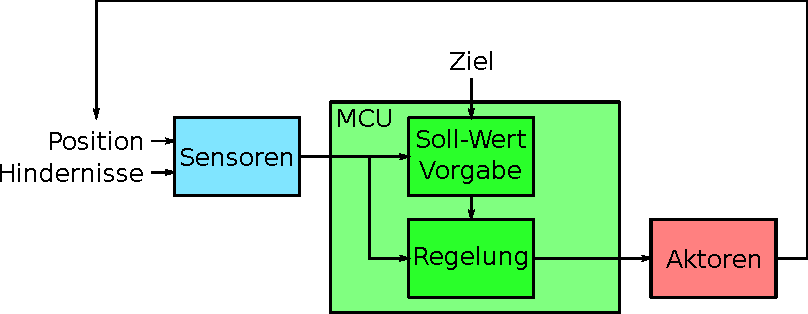
\includegraphics[width=\linewidth]{eva}
\end{frame}

\subsection{Selbstlokalisation}
\begin{frame}{\insertsection: \insertsubsection}
\begin{minipage}{0.45\linewidth}
	\begin{itemize}
		\item GPS
		\note{\textbf{GPS:}\\
			funktioniert nur im Freien\\
			lokal ungenau, global genau
		}
		\item Accelerometer
		\note{\\ \textbf{ACC:}\\
			funktioniert überall\\
			lokal genau, drift möglich
		}
		\item Gyroskop
		\item Magnetometer
		\item Kamera
		\note{\\ \textbf{Kamera:}\\
			Abgleich mit Umgebungsdatenbank
		}
	\end{itemize}
\end{minipage} \quad
\begin{minipage}{0.45\linewidth}
	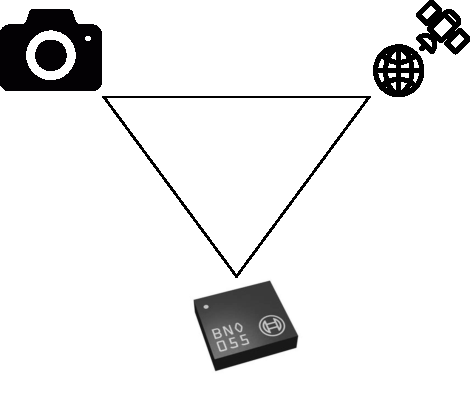
\includegraphics[width=\linewidth]{selbstlokalisation}
\end{minipage}
\end{frame}

\subsection{Kollisionsvermeidung}
\begin{frame}{\insertsection: \insertsubsection}
\begin{minipage}{0.35\linewidth}
	\begin{itemize}
		\item Ultraschall
		\note{\textbf{Ultraschall:}\\
			geringe Reichweite \\
			einfach \\
		}
		\item LIDAR
		\note{\textbf{LIDAR:}\\
			hohe Reichweite \\
			aufwendig \\
		}
		\item (Stereo-)Kamera
		\note{\textbf{Kamera:}\\
			Kollisionserkennung \\
		}
	\end{itemize}
\end{minipage} \quad
\begin{minipage}{0.55\linewidth}
	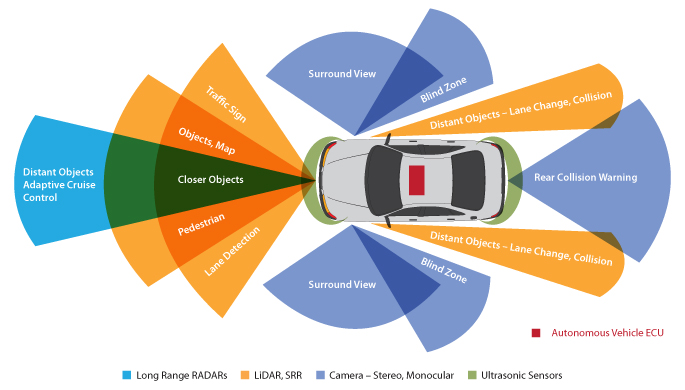
\includegraphics[width=\linewidth]{suto}
	
	{\tiny Quelle: http://www.tataelxsi.com/ip-solution/automotive/Autonomai.html}
\end{minipage}
\end{frame}

\subsection{Recheneinheiten}
\begin{frame}{\insertsection: \insertsubsection}
\begin{minipage}{0.35\linewidth}
	
	Entscheidungsfindung
	
	\begin{itemize}
		\item Trajektorienplanung
		\note{\\ \textbf{Trajektorienplanung:}
			Mikrocontroller wäre ausreichend
		}
		\item Neuronale Netze
		\note{\\ \textbf{Neuronale Netze:}
			Hohe Rechenintensität
		}
	\end{itemize}

	Weitere Aufgaben

	\begin{itemize}
		\item Sensorverarbeitung
		\item Regelung
		\note{\\ \textbf{Regelung:}
			Echtzeit-Anforderungen
		}
	\end{itemize}
\end{minipage} \quad
\begin{minipage}{0.55\linewidth}
	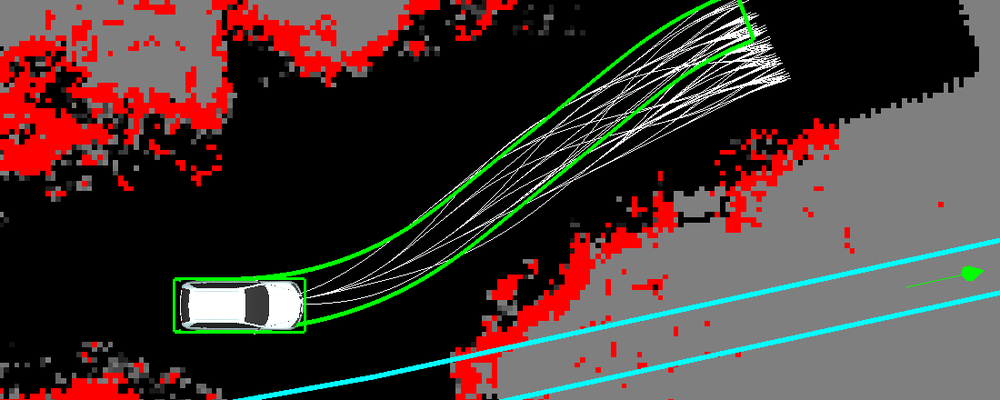
\includegraphics[width=\linewidth]{trajektorien}
	
	{\tiny Quelle: https://www.unibw.de/tas/forschung/trajektorienplanung/view}
\end{minipage}
\end{frame}

\subsection{Gemeinsamkeiten}
\begin{frame}{\insertsection: \insertsubsection}
\begin{table}
	\begin{tabular}{|l|c|c|}
		\hline
		& SEC-Bike & Boot \\ \hline
		GPS & $\checkmark$ & $\checkmark$ \\ \hline
		Accelerometer & $\checkmark$ & $\checkmark$ \\ \hline
		(Stereo-) Kamera & $\checkmark$ & \\ \hline
		Ultrschall & $\checkmark$ & $\checkmark$ \\ \hline
		LIDAR & $\checkmark$ & \\ \hline
		Trajektorienplanung & $\checkmark$ & $\checkmark$ \\ \hline
		Neuronale Netze & $\checkmark$ & \\ \hline
		Regelung & $\checkmark$ & $\checkmark$ \\ \hline
	\end{tabular}
\end{table}
\end{frame}

\section{Softwareplanung}
\subsection{Betriebssystem}
\begin{frame}{\insertsection: \insertsubsection}

\begin{itemize}
	\item Kein Betriebssystem
	\only<1>{
	\begin{itemize}
		\item Schwer erweiterbar
		\item Hoher Entwicklungsaufwand
	\end{itemize}}
	\item Free-RTOS
	\only<2>{
	\begin{itemize}
		\item Erfahrung war vorhanden
		\item Nicht auf EFM32 portiert.
	\end{itemize}}
	\item Robot Operating System (ROS)
	\only<3>{
	\begin{itemize}
		\item Für diesen Anwendungsfall entwickelt
		\item Kein EFM32-Port verfügbar
		\note{ROS: Basiert auf Linux, nicht genügend Performance vorhanden}
	\end{itemize}}
	\item Micrium-OS
	\only<4>{
	\begin{itemize}
		\item Empfohlen von Silicon Laboratories
		\item Port auf EFM32 und EFR32 vorhanden.
	\end{itemize}}
	\note{
		Betriebssystem abstrahiert Hardware \\
		Betriebssystem verfügt über Scheduler. Dieser ermöglicht Multitasking.\\
		Entscheidung fiel auf MicriumOS, da es als einziges einen Port für die Controller hat. \\
		Zeitaufwand für Entwicklung eines eigenen Ports zu hoch.
	}
\end{itemize}
\end{frame}

\subsection{Aufgaben}
\begin{frame}{\insertsection: \insertsubsection}

	Anwendungsfall Sonarboot

	\includegraphics[width=\linewidth]{aufgaben1}

\end{frame}

\begin{frame}{\insertsection: \insertsubsection}

	Anwendungsfall SEC-Bike

	\includegraphics[width=\linewidth]{aufgaben2}

\end{frame}

\section{Hardwarearchitektur}
\subsection{Recheneinheiten}

\begin{frame}{\insertsection: \insertsubsection}

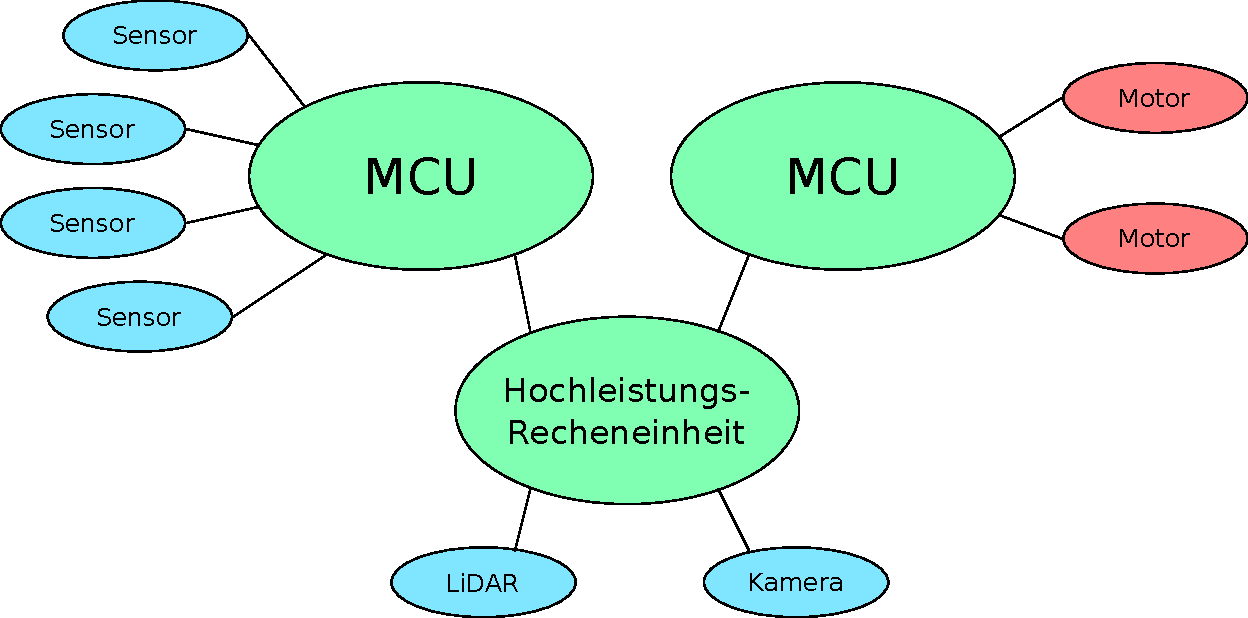
\includegraphics[width=\linewidth]{aufgaben_mcu}

\end{frame}

\subsection{Sensoren}
\begin{frame}{\insertsection: \insertsubsection}	
	Lokalisation und Kollisionsvermeidung
	\begin{itemize}
		\item Beschleunigungssensor (9DOF)
		\item GPS
		\item Drucksensor
		\note{Drucksensor zur Höhenangabe}
		\item Drehgeber
		\item Ultraschall
	\end{itemize}
\end{frame}

\subsection{Aktoren}
\begin{frame}{\insertsection: \insertsubsection}
\begin{minipage}{0.45\linewidth}
	
	\begin{itemize}
		\item CAN-Interface
		\item Servo-Signal
		\item Audioausgabe
	\end{itemize}
\end{minipage} \quad
\begin{minipage}{0.45\linewidth}
	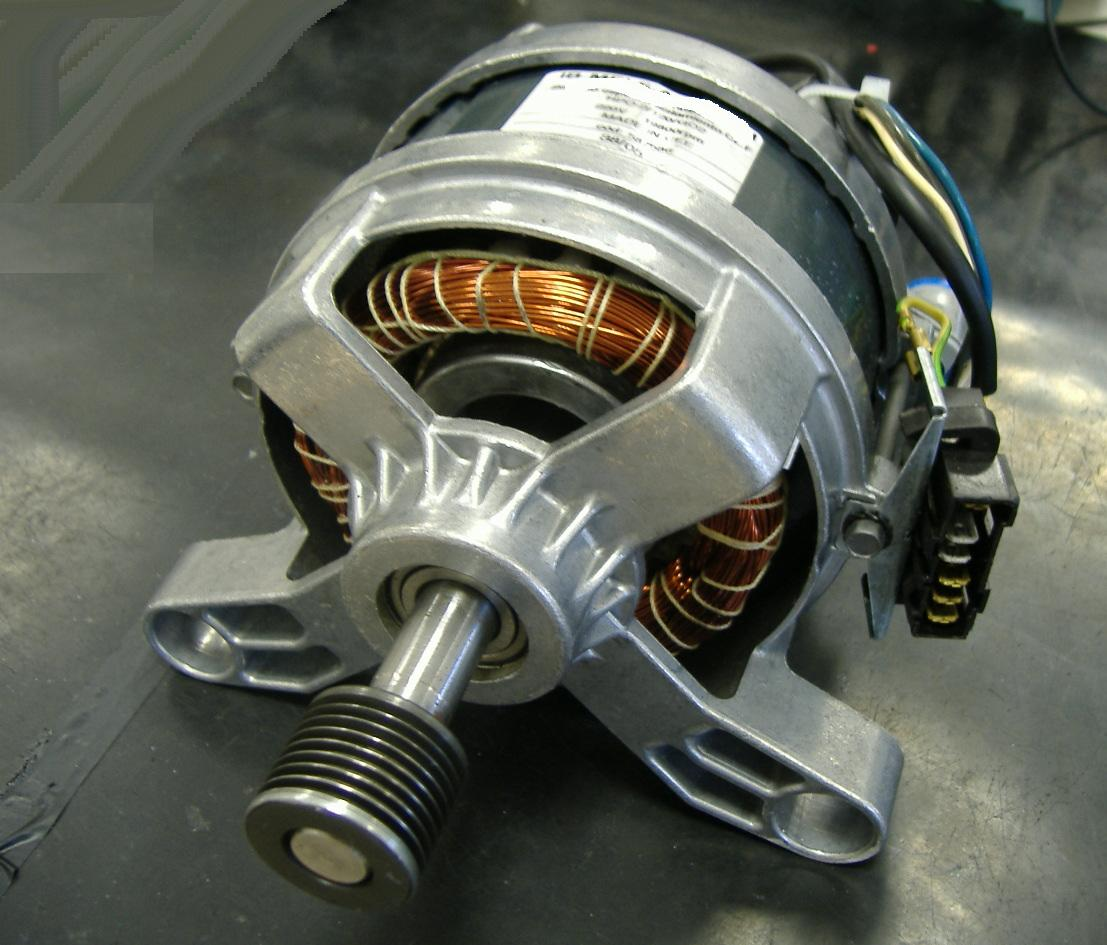
\includegraphics[width=\linewidth]{motor}
\end{minipage}
\end{frame}

\subsection{Debug- und Steuer-Optionen}
\begin{frame}{\insertsection: \\ \insertsubsection}
\begin{minipage}{0.45\linewidth}
	\begin{itemize}
		\item USB-UART-Bridge
		\item SD-Karte
		\note{SD-Karte: speichern von Sensor-Roh-Daten}
		\item MightyGecko-Funkverbindung
		\item Servo-Eingänge
	\end{itemize}
\end{minipage} \quad
\begin{minipage}{0.45\linewidth}
	\centering
	\begin{tabular}{c c c}
		
\includegraphics[width=0.2\linewidth]{usb-symbol} & 
		
\includegraphics[width=0.2\linewidth]{sd-card} & 
		
\includegraphics[width=0.2\linewidth]{bluetooth} \\
		\hspace{0.3 \linewidth} & \hspace{0.3 \linewidth} & \hspace{0.3 \linewidth} \\
	\end{tabular}
\end{minipage}
\end{frame}

\subsection{Stromversorgung}
\begin{frame}{\insertsection: \insertsubsection}
\begin{minipage}{0.45\linewidth}
	\begin{itemize}
		\item Weiter Eingangsspannungsbereich
		\note{Eingangsspannungsbereich: 7V to 75V}
		\item Stromversorgung für Onboard-Elektronik
		\item Unabhängiger Schaltregler
		\item Batteriemanagement extern
	\end{itemize}
\end{minipage} \quad
\begin{minipage}{0.45\linewidth}
	\includegraphics[width=\linewidth]{stromversorgung}
\end{minipage}
\end{frame}

\subsection{Mikrocontroller}
\begin{frame}{\insertsection: \insertsubsection}
\begin{minipage}{0.45\linewidth}
	
	Sensorverarbeitung
	
	\begin{itemize}
		\item SiLabs GiantGecko GG11
		\begin{itemize}
			\item Große Auswahl an Peripherie
			\item 72 MHz Cortex-M4 mit FPU
		\end{itemize}
	\end{itemize}

\end{minipage} \quad
\begin{minipage}{0.45\linewidth}
	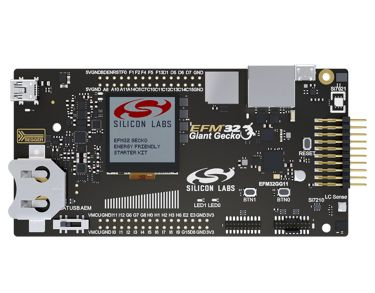
\includegraphics[width=\linewidth]{efm32}
\end{minipage}
\end{frame}

\begin{frame}{\insertsection: \insertsubsection}
\begin{minipage}{0.45\linewidth}

	Regelung
	\begin{itemize}
		\item SiLabs MightyGecko MG12
		\begin{itemize}
			\item Aufsteckmodul
			\item Verschiedene Funkstandards
			\item 40 MHz Cortex-M4 mit FPU
		\end{itemize}
	\end{itemize}
\end{minipage} \quad
\begin{minipage}{0.45\linewidth}
	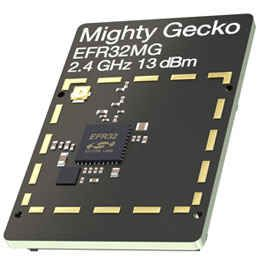
\includegraphics[width=\linewidth]{efr32}
\end{minipage}
\end{frame}

\subsection{Übersicht}
\begin{frame}{\insertsection: \insertsubsection}
	\centering
	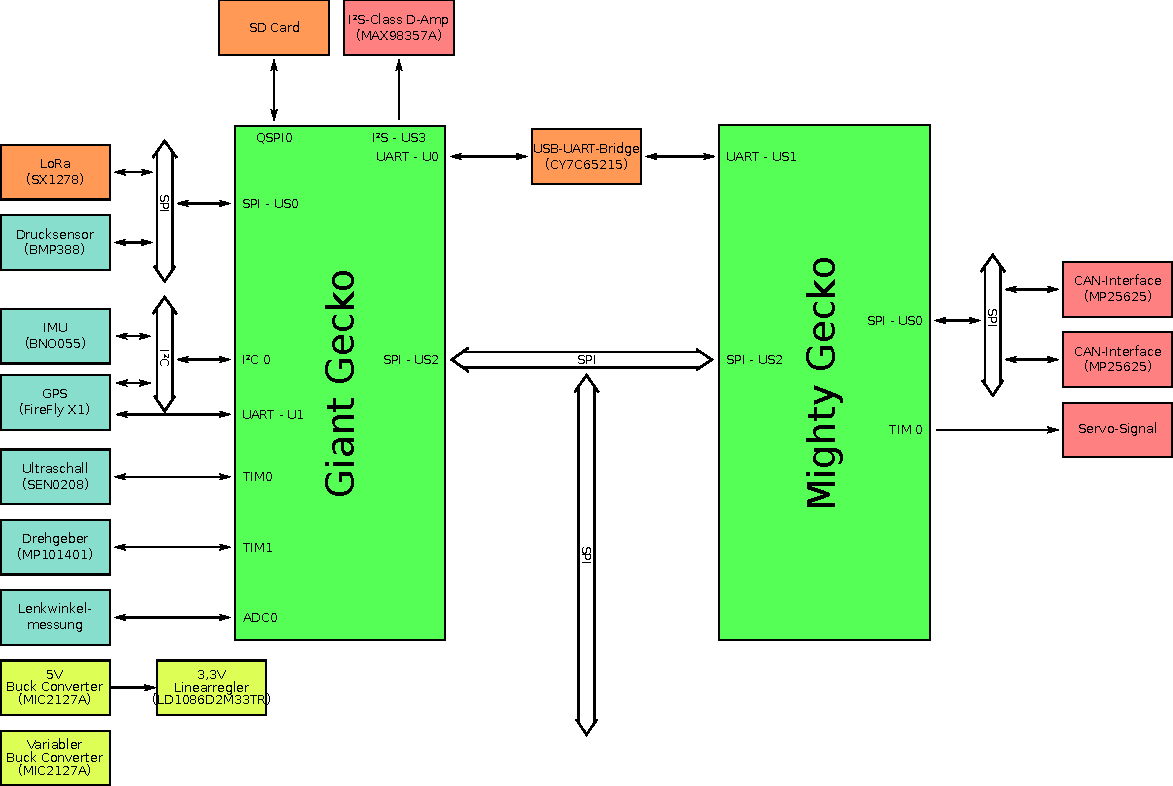
\includegraphics[width=0.9\linewidth]{architecture_detailed}
\end{frame}

\section{Softwarearchitektur}

\subsection{Anwendungsfall Boot}
\begin{frame}{\insertsection: \insertsubsection}
\begin{minipage}{0.45\linewidth}
	\begin{itemize}
		\item Sensorauswertung im Giant Gecko
		\item Trajektorienplanung und Regelung im Mighty Gecko
		\item Sonardaten werden unabhängig verarbeitet
	\end{itemize}
\end{minipage} \quad
\begin{minipage}{0.45\linewidth}
	\includegraphics[width=\linewidth]{microcontrollers}
\end{minipage}
\end{frame}

\subsection{Anwendungsfall SEC-Bike}
\begin{frame}{\insertsection: \insertsubsection}
\begin{minipage}{0.45\linewidth}
	\begin{itemize}
		\item Sensorauswertung im Giant Gecko
		\item Auswertung komplexer Sensoren und Entscheidung in externer Hochleistungsrecheneinheit
		\item Regelung im Mighty Gecko
	\end{itemize}
\end{minipage} \quad
\begin{minipage}{0.45\linewidth}
	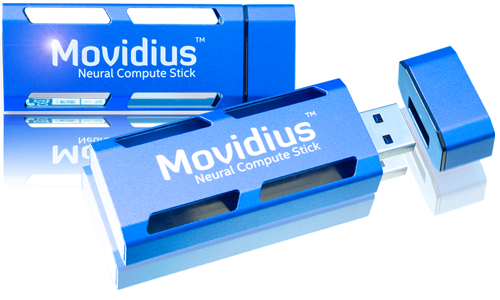
\includegraphics[width=\linewidth]{movidius}
\end{minipage}
\end{frame}

\subsection{Giant Gecko}
\begin{frame}{\insertsection: \insertsubsection}
	\begin{center}
		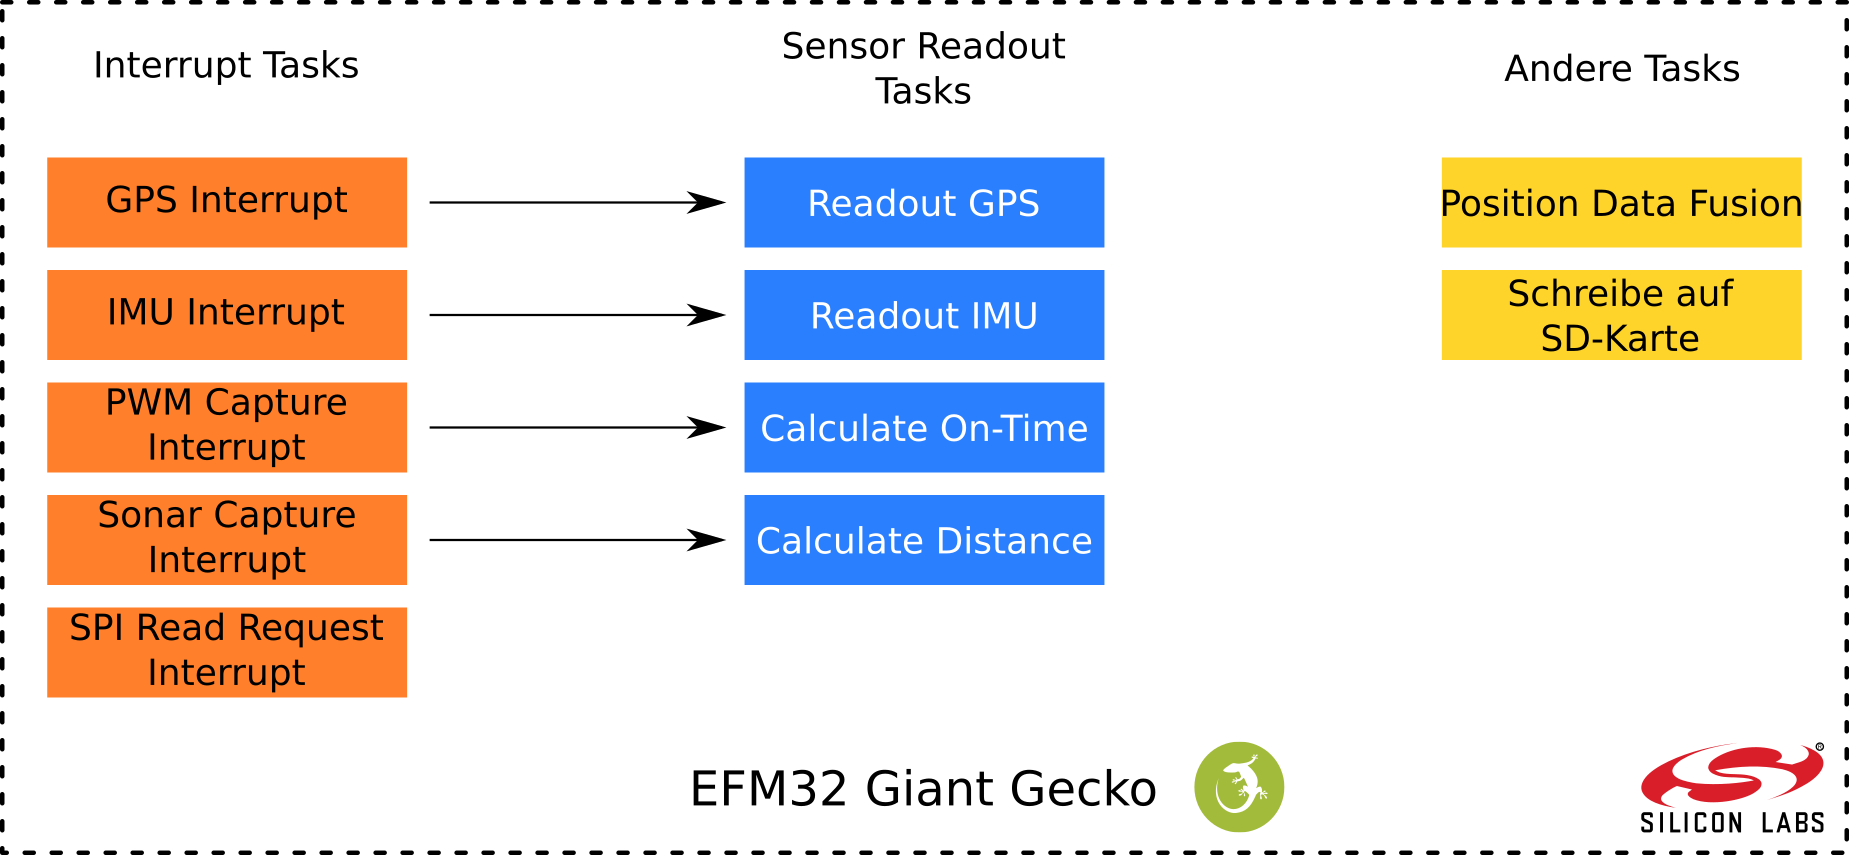
\includegraphics[width=0.9\linewidth]{gg_software_architecture}
	\end{center}
	
	Basiert auf Echtzeitbetriebssystem Micrium OS
\end{frame}

\subsection{Mighty Gecko}
\begin{frame}{\insertsection: \insertsubsection}

	\begin{center}
		{\Huge To Be Defined} 
		
		{\Huge ?}
	\end{center}

Basiert auf Echtzeitbetriebssystem Micrium OS
\end{frame}

\section{Aktueller Stand}
\subsection{Hardware}
\begin{frame}{\insertsection: \insertsubsection}
\begin{minipage}{0.45\linewidth}
	\begin{itemize}
		\item Platine entwickelt
		\item Bauteile bestellt
		\item Platine teilweise bestückt
	\end{itemize}
\end{minipage} \quad
\begin{minipage}{0.45\linewidth}
	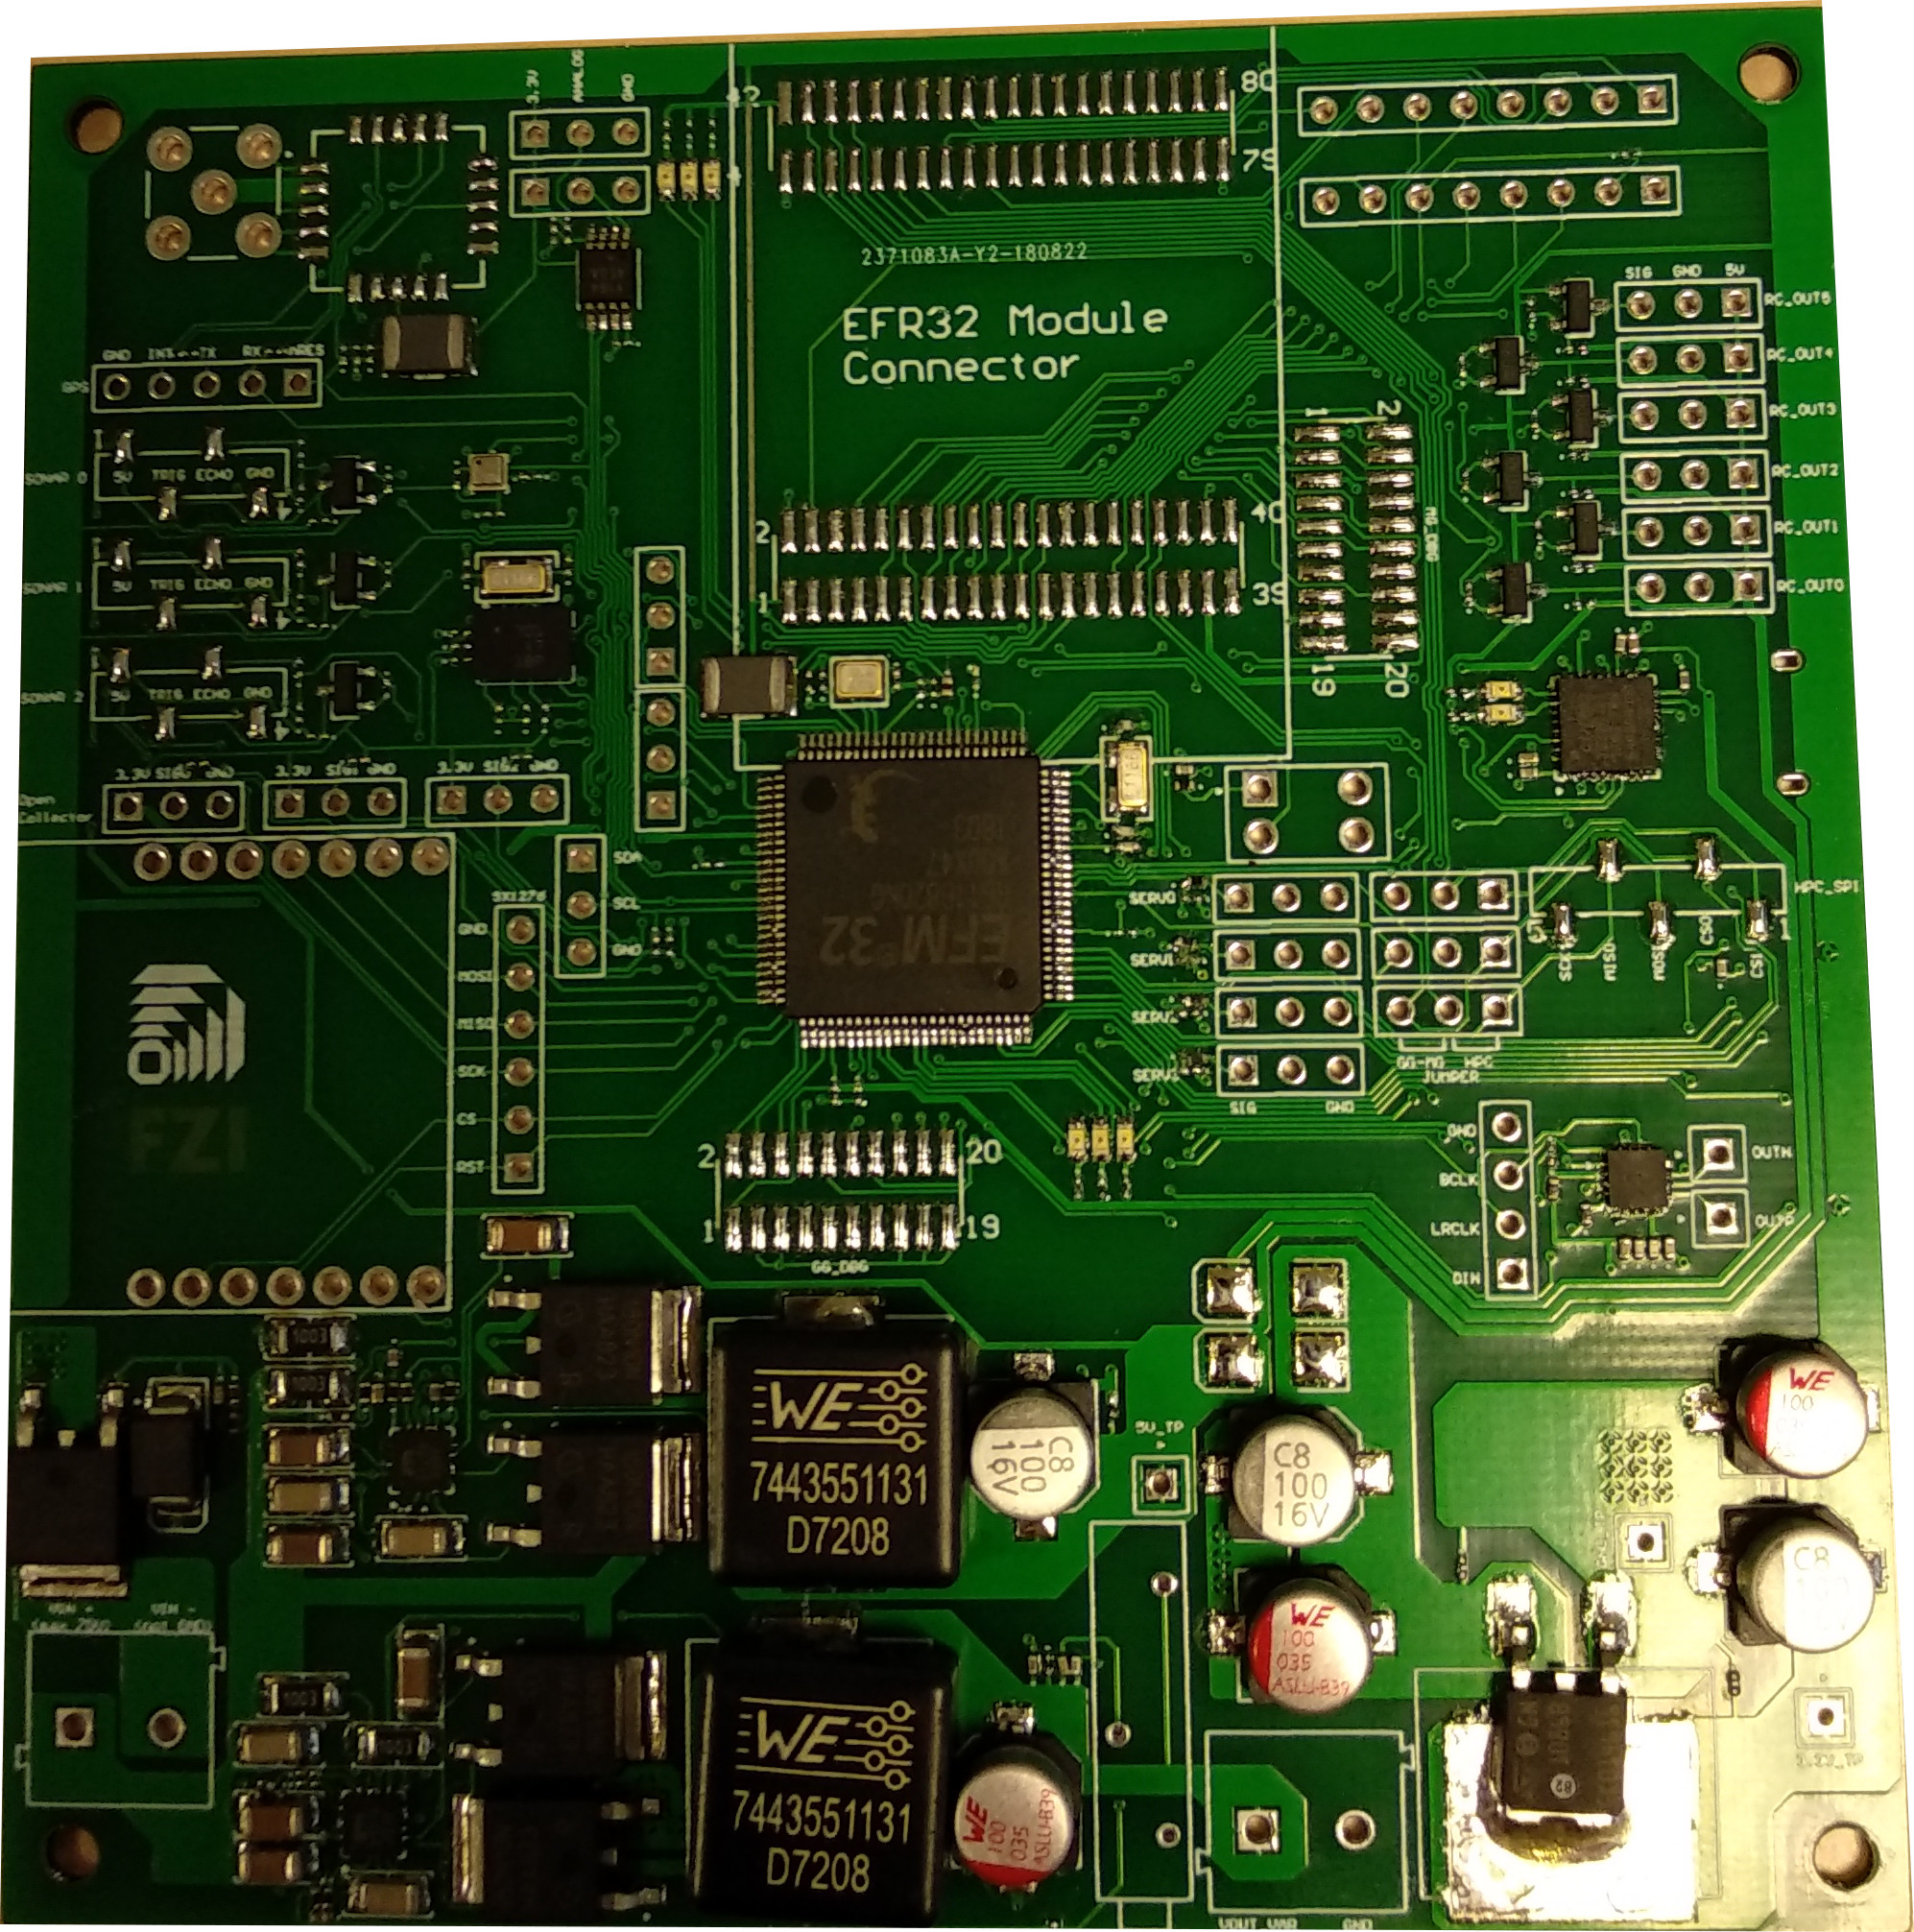
\includegraphics[width=\linewidth]{platine2}
\end{minipage}
\end{frame}

\subsection{Software}
\begin{frame}{\insertsection: \insertsubsection}
	\begin{itemize}
		\item Architektur für Sensordatenverarbeitung entwickelt
		\item IMU mit Entwicklungsboard in Betrieb genommen
	\end{itemize}
\end{frame}

\subsection{GANTT-Diagramm}
\begin{frame}{\insertsection: \insertsubsection}

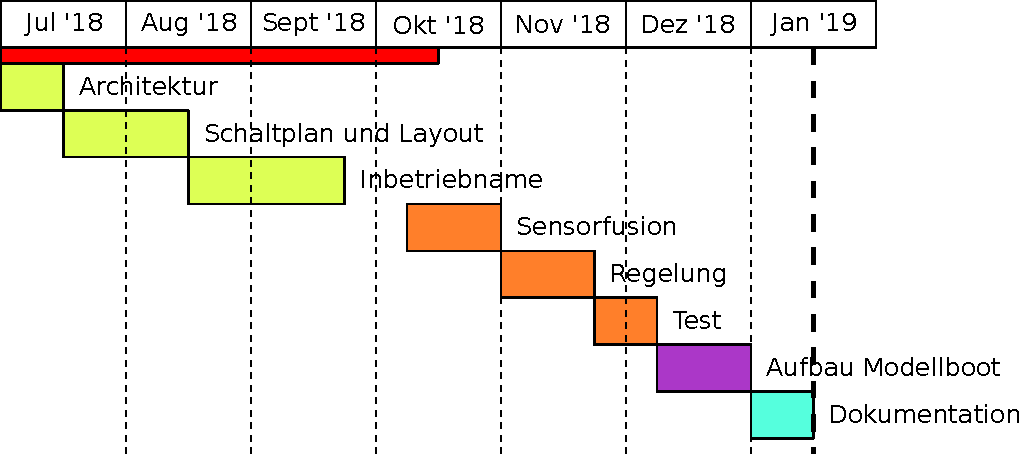
\includegraphics[width=\linewidth]{gantt}

\end{frame}

\section{Aussicht}

\subsection{Ziele}
\begin{frame}{\insertsection: \insertsubsection}
\begin{minipage}{0.45\linewidth}
	\begin{itemize}
		\item Minimum an Sensoren
		\begin{itemize}
			\item GPS
			\item IMU
		\end{itemize}
		\item einfache Pfadverfolgung
		\item Modellboot-Demonstrator
	\end{itemize}
\end{minipage} \quad
\begin{minipage}{0.45\linewidth}
	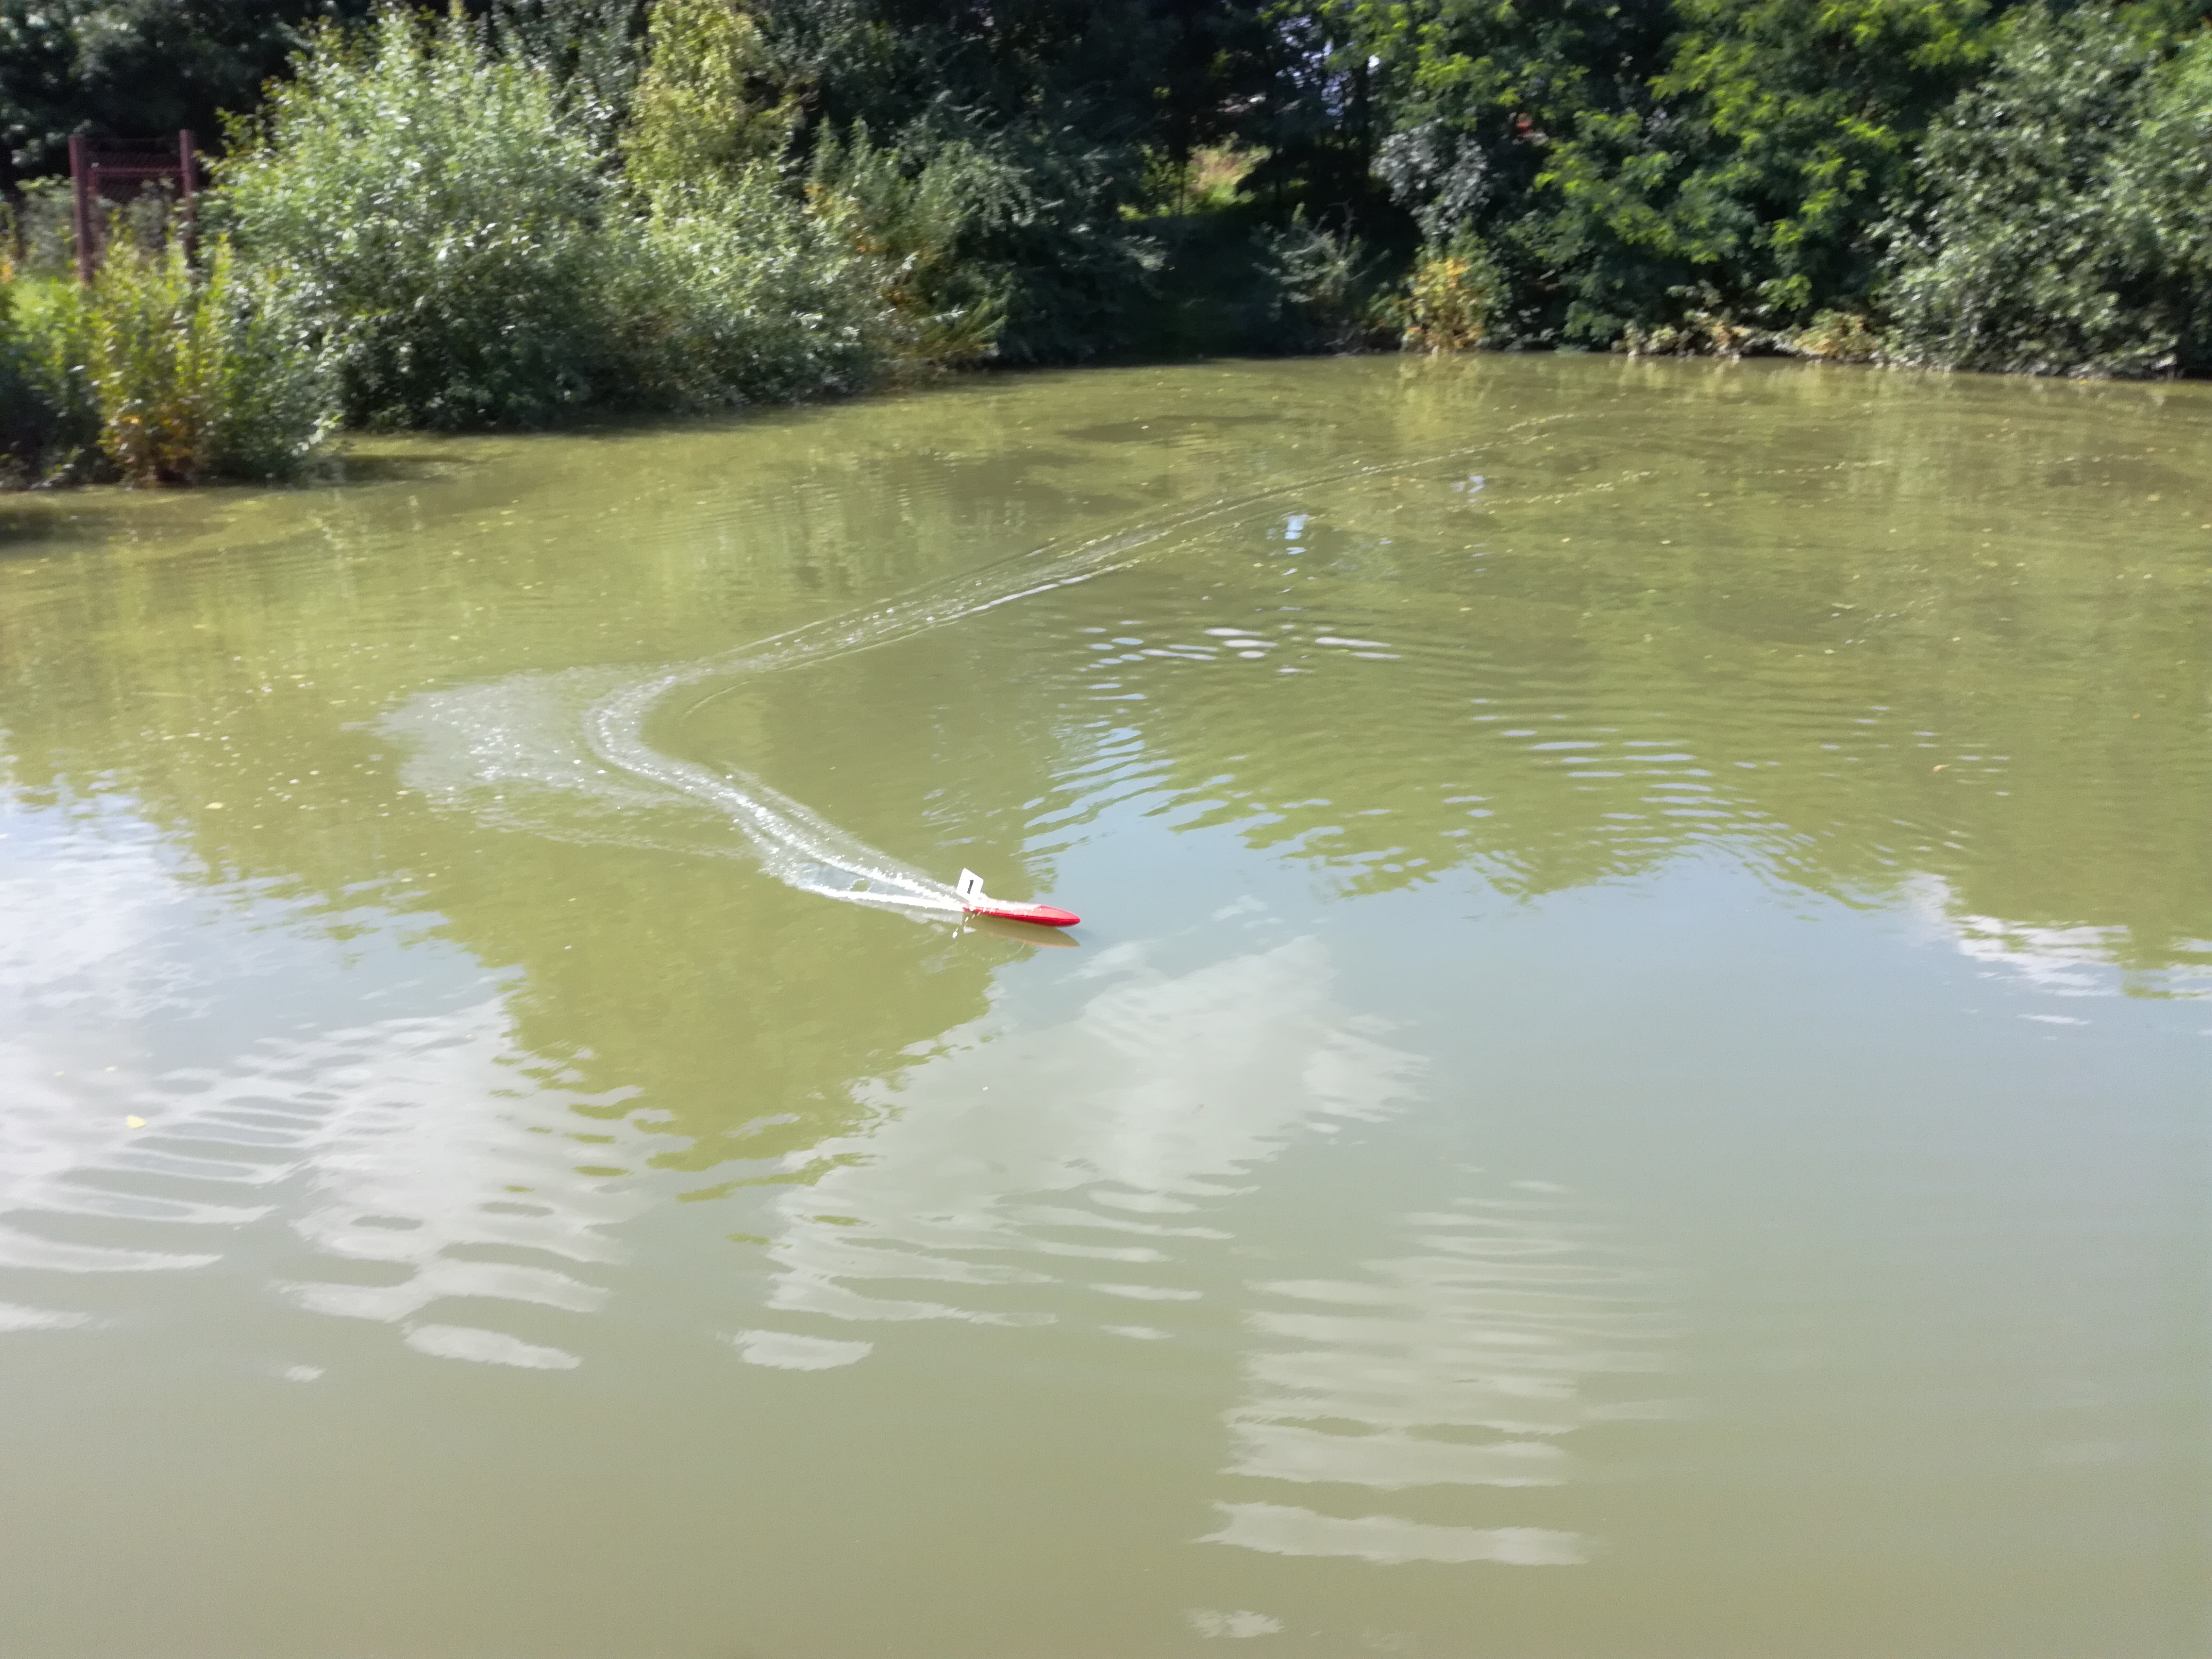
\includegraphics[width=\linewidth]{rc-boat}
\end{minipage}
\end{frame}

\subsection{Verwendung}
\begin{frame}{\insertsection: \insertsubsection}
\begin{minipage}{0.45\linewidth}
	\begin{itemize}
		\item Basis verschiedener Kleinfahrzeuge
		\item Hardware generisch
		\item Software erweiterbar
		\item Platine 10cm x 10cm
	\end{itemize}
\end{minipage} \quad
\begin{minipage}{0.45\linewidth}
	\includegraphics[width=\linewidth]{logos/platine}
\end{minipage}
\end{frame}

\end{document}